\documentclass{beamer}
\usepackage[utf8]{inputenc}
\usepackage[french]{babel}
\usepackage{graphics}
\usepackage{tabularx}
\usepackage[french]{babel}
\usepackage[T1]{fontenc}
\usepackage{libertine}


%\usepackage[screen,nopanel]{pdfscreen}
%\usepackage{url}

\usetheme[progressbar=frametitle,numbering=none]{metropolis}
\definecolor{Pourpre}{RGB}{174,37,115} 
\setbeamercolor{alerted text}{fg=Pourpre}
%\setbeamertemplate{itemize items}{\textcolor{Pourpre}{\footnotesize$\blacksquare$}}

\title{Initiation et développement de l'agilité en DUT Informatique}
\author[Thomas Clavier, Yann Secq]
{
  \{ \textbf{Thomas.Clavier \& Yann.Secq} \}\texttt{@univ-lille1.fr}
}
\institute{
  
\includegraphics[height=13mm]{includes/logo_iut_A_Lille.jpg}
  
\includegraphics[height=13mm]{includes/logo_Univ_de_Lille.jpg}
}
  
\date{}

\logo{
    
\includegraphics[width=1cm]{includes/CC_BY_SA} 
}

\begin{document}

\frame{\titlepage}

\begin{frame}{Bipodocratie}
  \begin{columns}
    \begin{column}{0.5\textwidth}
      \begin{center}
        
\includegraphics[width=0.6\textwidth]{includes/foots.png}      
      \end{center}
    \end{column}
    \begin{column}{0.5\textwidth}
      Si vous n’apprenez rien ou que vous ne contribuez pas, suivez vos pieds !
    \end{column}
  \end{columns}
\end{frame}

\section{Introduction}
\begin{frame}{Enseignement de l'agilité à l'Université}
Tribulations à l'Université d'un agiliste professionnel et de son compère enseignant-chercheur en quête d'une révolution de la pédagogie académique
   \begin{itemize}
     \item Pourquoi de l'agilité en DUT ?
     \item Comment tout a démarré
     \item Des petits pas
     \item Et maintenant ?
   \end{itemize}
\end{frame}

\begin{frame}{Pourquoi de l'agilité en DUT}
   \begin{itemize}
    \item DUT, une fabrique de développeurs
    \item Contact direct et (assez) étroit avec les réalités professionnelles
    \item Info: algorithmique et programmation, système et réseau, base de données, méthodologie et analyse
    \item Enseignement académique $\Rightarrow$ silos disciplinaires :(
    \item Réforme du PPN en 2013 $\Rightarrow$ projet de semestre
   \end{itemize}
\end{frame}

\begin{frame}{Comment tout a démarré}
   \begin{itemize}
     \item Un réseau national structuré ...
     \item Les <<grandes>> Journées Agiles(Toulouse'12, Aix'13, Montreuil'14)
     \item Les <<petites>> Journées Agiles (\textbf{Lille'13}, Lyon'14)
     \item Premier poste de PAST au département pour septembre 2013 !
     \item Début des projets sur la lune pour Laurel et Hardy
   \end{itemize}
\end{frame}

{
\usebackgroundtemplate{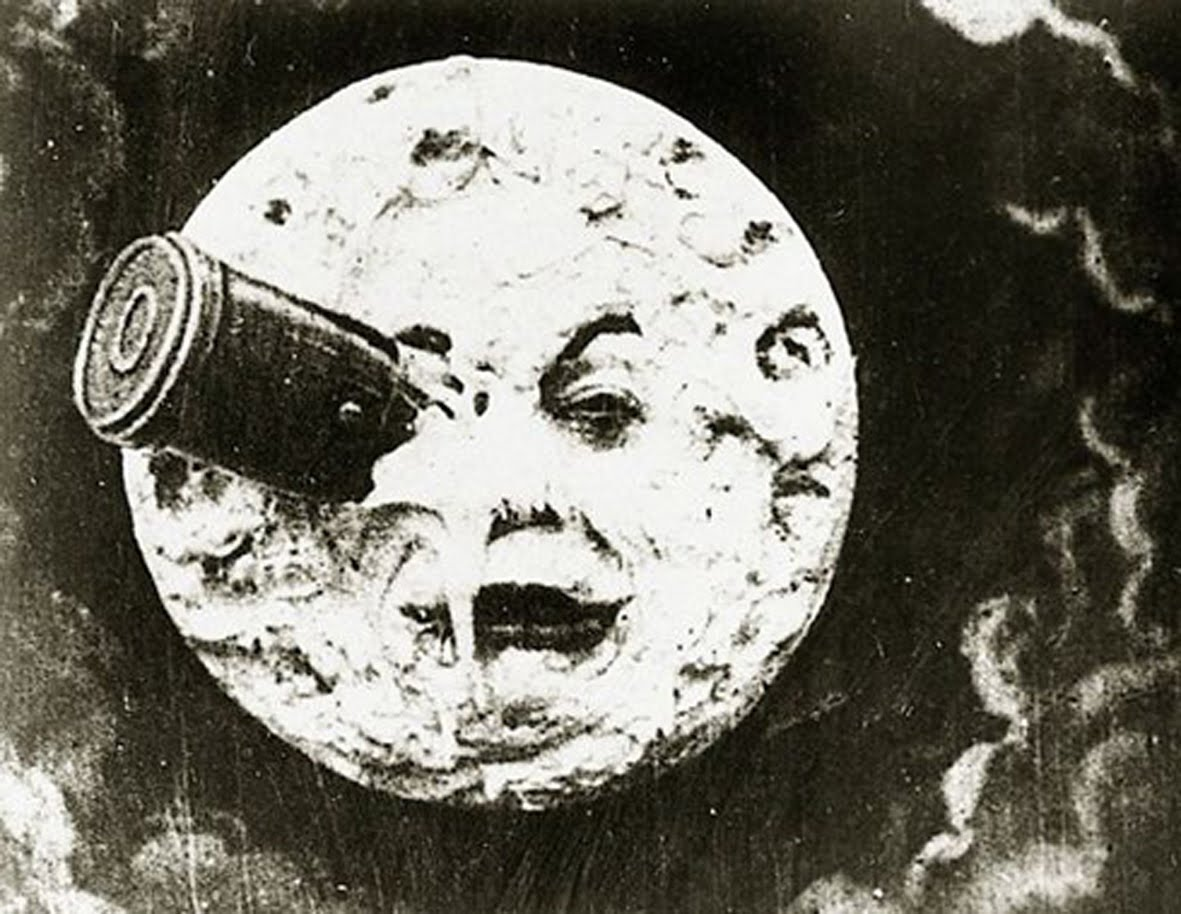
\includegraphics[width=\paperwidth]{includes/le-voyage-dans-la-lune-oeil.jpg}}
\begin{frame}[plain]
\end{frame}
}

\section{Janvier 2014}
\subsection{Objectifs}
\begin{frame}{Janvier 2014 : Objectifs}
  %Premier projet agile, un groupe de S3.

  \begin{itemize}
    \item découvrir l'agilité et l'amélioration continue à travers un projet 
    \item prototyper rapidement un produit web avec un serveur REST du JS, html et bootstrap
    \item prouver aux collègues que c'est possible.
  \end{itemize}
\end{frame}

\subsection{Deroulement}
\begin{frame}{Janvier 2014 : Déroulement}
  \begin{itemize}
    \item 2 encadrants pour un groupe de TP
    \item auto-organisation des équipes de 6 ou 7
    \item des sujets apportés par les étudiants
    \item des contraintes techniques fortes
  \end{itemize}
\end{frame}

\begin{frame}{Janvier 2014 : Planning}
  \begin{center}
    \begin{tabular}{| c | c | c |}
      \hline
      \textbf{Jour 1} & \textbf{Jour 2} & \textbf{Jour 3} \\
      \hline \hline
      Lego4scrum & sprint & sprint        \\
      \hline
                 & sprint & sprint        \\
      \hline \hline
      backlog    & sprint & soutenance    \\
      \hline
      sprint 0   & sprint & rétrospective \\
      \hline
    \end{tabular}
  \end{center}
  2h de sprint = 1h30 de code + démo + rétro
\end{frame}

\subsection{Apprentissages}
\begin{frame}{Janvier 2014 : Apprentissages}
  \begin{columns}
    \begin{column}{0.5\textwidth}
      \begin{center}
        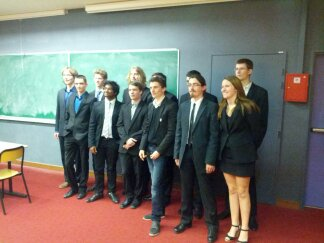
\includegraphics[width=\textwidth]{includes/201401_soutenance.jpg}      
      \end{center}
    \end{column}
    \begin{column}{0.5\textwidth}
  \begin{itemize}
    \item 1 enseignant pour 13 étudiants c'est parfait
    \item la généralisation à toute la promo est possible
    \item stress + bases théorique = apprentissage éclaire
    \item trop court.
  \end{itemize}
    \end{column}
  \end{columns}
\end{frame}

%\begin{frame}{Année 1 (septembre 2013 à juillet 2014)}
%  \begin{itemize}
%    \item de 96h théoriques à XXh pour l'agilité ...
%    \item \textbf{Problématique:} \emph{proof of concept}
%    \item première expérimentation: à petite échelle
%        \begin{itemize}
%          \item le groupe "PE" de 26 étudiants
%          \item constitution des équipes par les enseignants
%          \item 3 jours entre le S3 et le S4 (impact collègues)
%          \item sprint de 1h30 + 15mn démo + 15mn rétro
%          \item restitution et démo finale \emph{(plus sûr de ça !)}
%          \item rétrospective \textbf{très} enthousiaste des étudiants :)
%        \end{itemize}
%    \item \textbf{Objectif n+1}: généralisation à toute la promotion de S3 !
%  \end{itemize}
%\end{frame}

\section{Octobre 2014}
\subsection{Objectifs}
\begin{frame}{Octobre 2014 : Objectifs}
  Fin de S4 décalé avec la même recette qu'en S3 
  \begin{columns}
    \begin{column}{0.5\textwidth}
      \begin{center}
        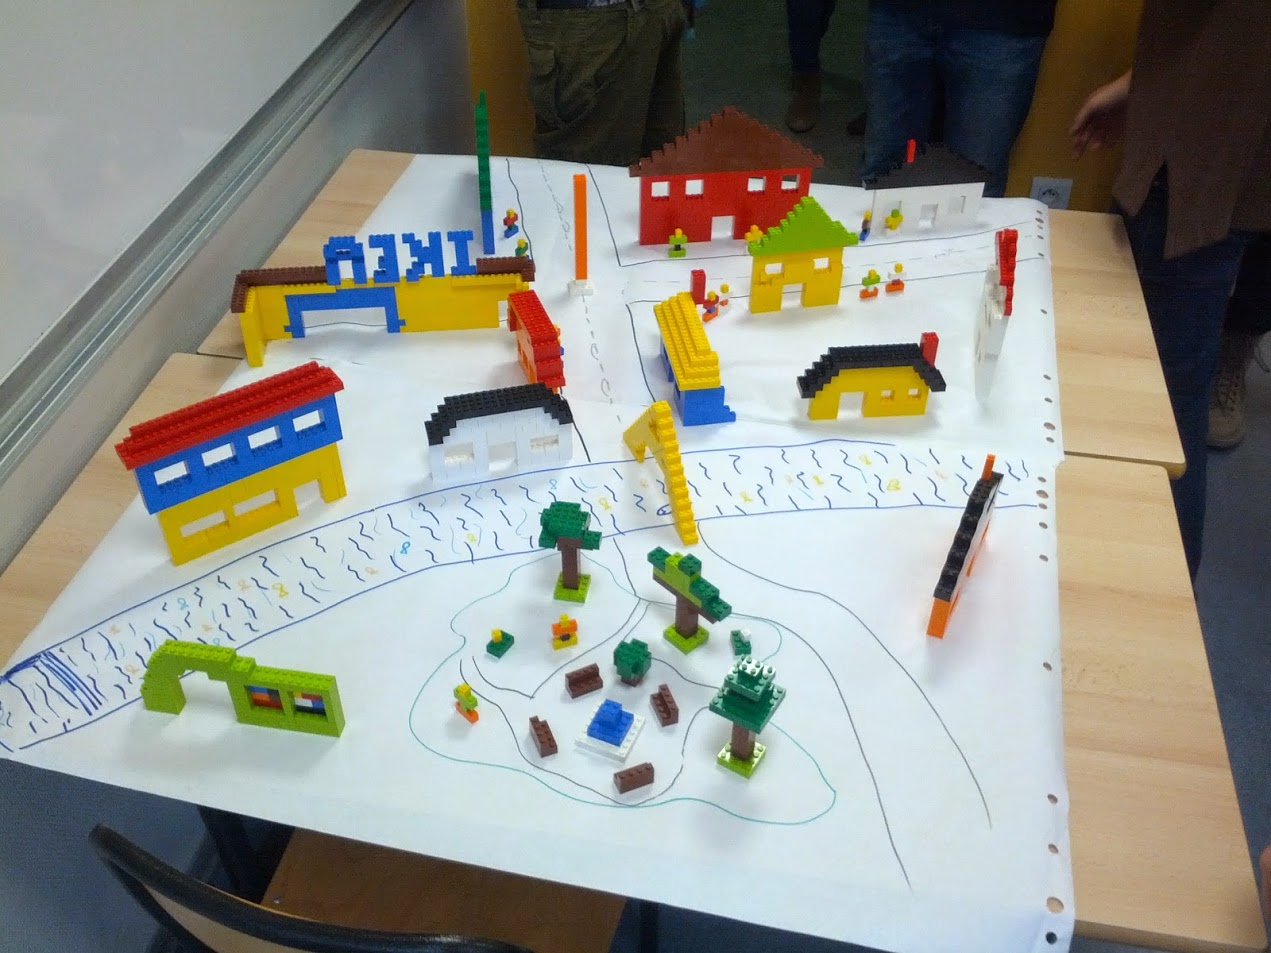
\includegraphics[width=\textwidth]{includes/201410_lego.jpg}      
      \end{center}
    \end{column}
    \begin{column}{0.5\textwidth}
      Objectifs : 
      \begin{itemize}
        \item valider la faisabilité d'une soutenance sous forme de salon 
        \item et l'adéquation avec la fin de formation
      \end{itemize}
    \end{column}
  \end{columns}
\end{frame}

\subsection{Apprentissages}
\begin{frame}{Octobre 2014 : Apprentissages}
  \begin{columns}
    \begin{column}{0.5\textwidth}
      \begin{center}
        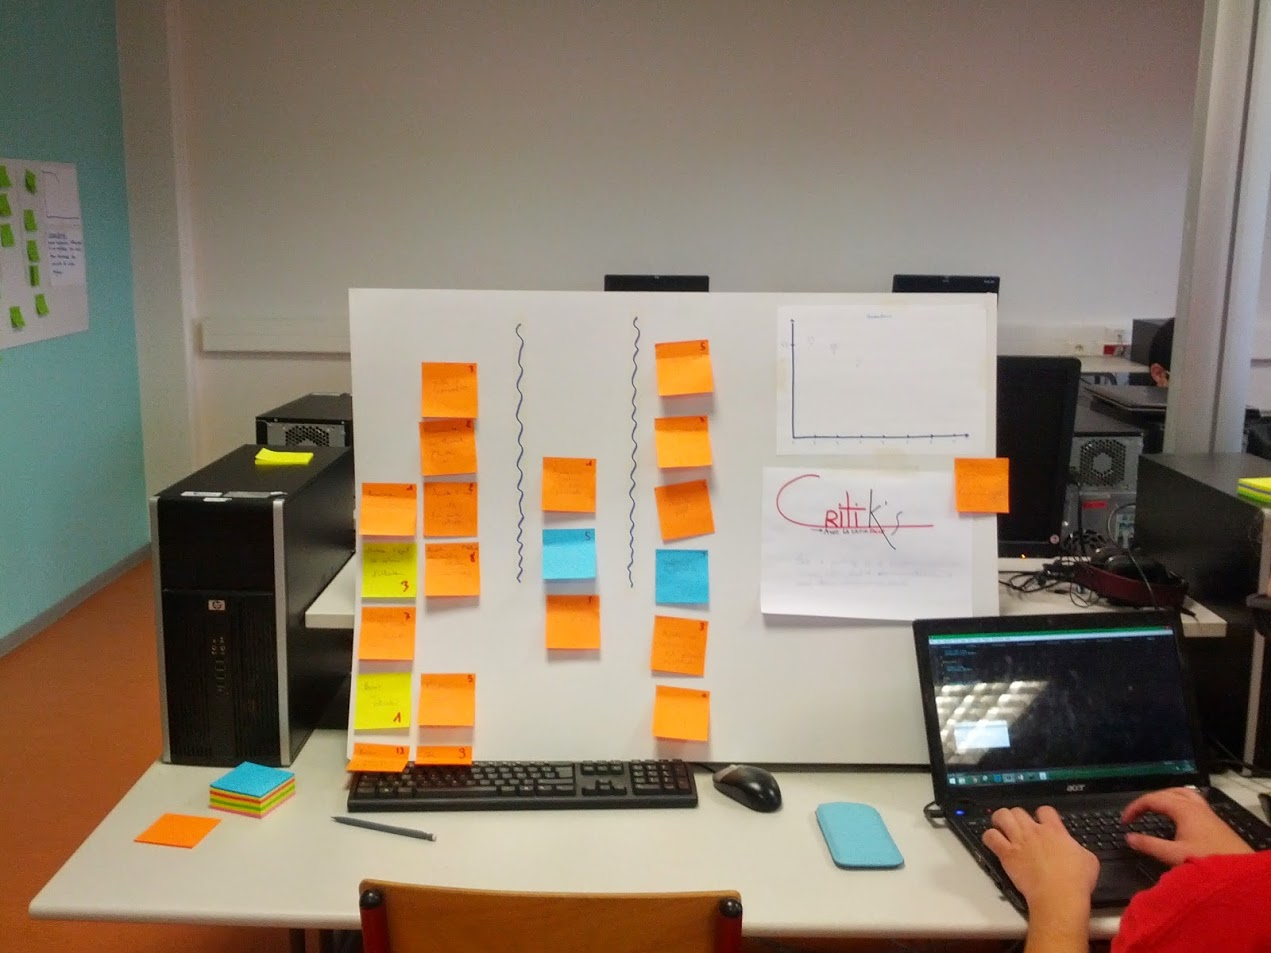
\includegraphics[width=\textwidth]{includes/201410_dashboard.jpg}      
      \end{center}
    \end{column}
    \begin{column}{0.5\textwidth}
      \begin{itemize}
        \item 1 enseignant pour 26 étudiants c'est très fatiguant,
        \item le salon pour la soutenance c'est ok.
      \end{itemize}
    \end{column}
  \end{columns}
\end{frame}

\section{Janvier 2015}
\subsection{Objectifs}
\begin{frame}{Janvier 2015 : Expérience}
  Toute la promo entre la fin du S3 et le début du S4, on vole une semaine de congé.
  \begin{columns}
    \begin{column}{0.5\textwidth}
      \begin{center}
        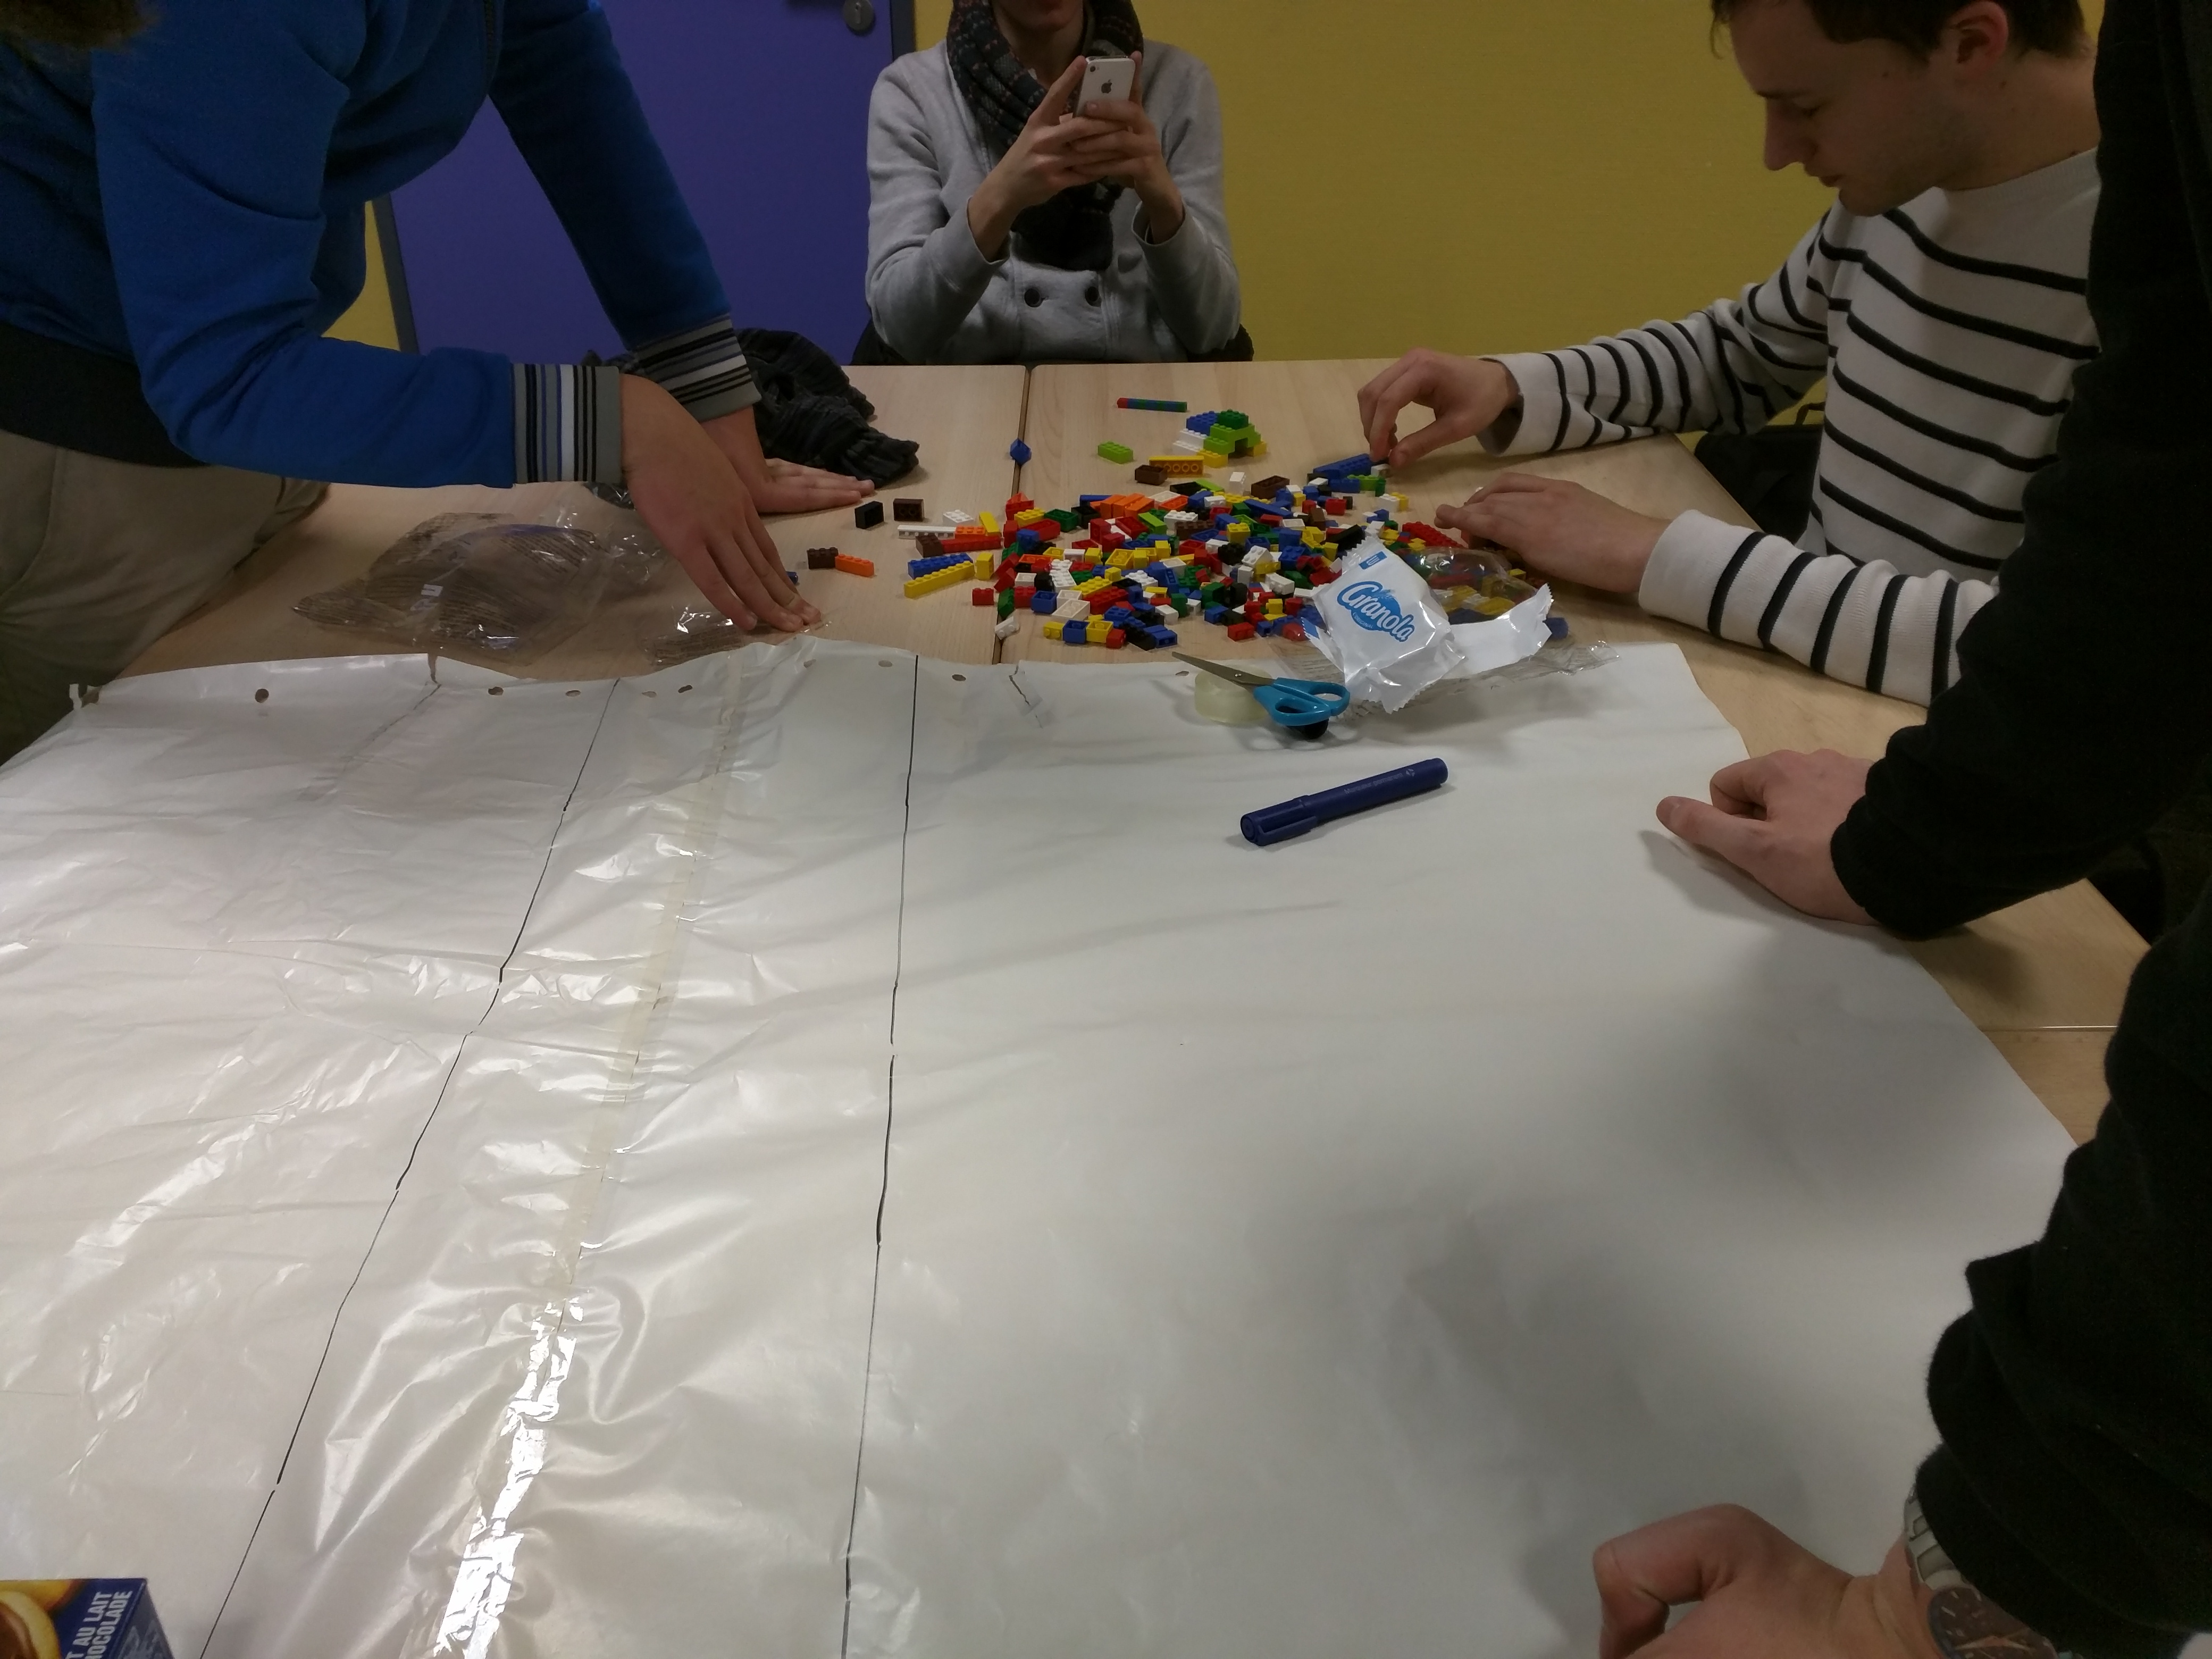
\includegraphics[width=\textwidth]{includes/201501_lego.jpg}      
      \end{center}
    \end{column}
    \begin{column}{0.5\textwidth}
      Objectifs : 
      \begin{itemize}
        \item valider le passage à l'échelle, 
        \item impliquer des collègues
      \end{itemize}
    \end{column}
  \end{columns}
\end{frame}

\subsection{Déroulement}
\begin{frame}{Janvier 2015 : Déroulement}
  \begin{itemize}
    \item 4 encadrants pour 4 groupes de TP.
    \item constitution des équipes par les enseignants
    \item 2 équipes issues de la journée entreprenariat
    \item des sujets apportés par les étudiants
    \item les mêmes contraintes technique
  \end{itemize}
\end{frame}

\begin{frame}{Janvier 2015 : Planning}
  \begin{center}
    \begin{tabular}{| c | c | c | c | c |}
      \hline
      \textbf{Jour 1} & \textbf{Jour 2} & \textbf{Jour 3} & \textbf{Jour 4} & \textbf{Jour 5} \\
      \hline \hline
      Lego4scrum      & sprint          & sprint          & sprint          & sprint          \\
      \hline
                      & sprint          & sprint          & sprint          & sprint          \\
      \hline \hline
      backlog         & sprint          & sprint          & sprint          & salon           \\
      \hline
      sprint 0        & sprint          & pitch           & sprint          & rétrospective   \\
      \hline
    \end{tabular}
  \end{center}
\end{frame}

\subsection{Apprentissages}
\begin{frame}{Janvier 2015 : Apprentissages}
  \begin{itemize}
    \item les enseignants non agiliste sont en difficultés
    \item la généralisation est un succès
    \item les étudiants sont enthousiastes
    \item ça génère une cohésion de promotion extraordinaire
    \item 5 jours d'affilé c'est éprouvant
    \item il faut tester plus tard dans l'année.
  \end{itemize}
\end{frame}

\section{Septembre 2015}
\subsection{Objectifs}
\begin{frame}{Septembre 2015 : Expérience}
  Toute la promo en début de S3 : FI et FC.

  \begin{columns}
    \begin{column}{0.5\textwidth}
      \begin{center}
        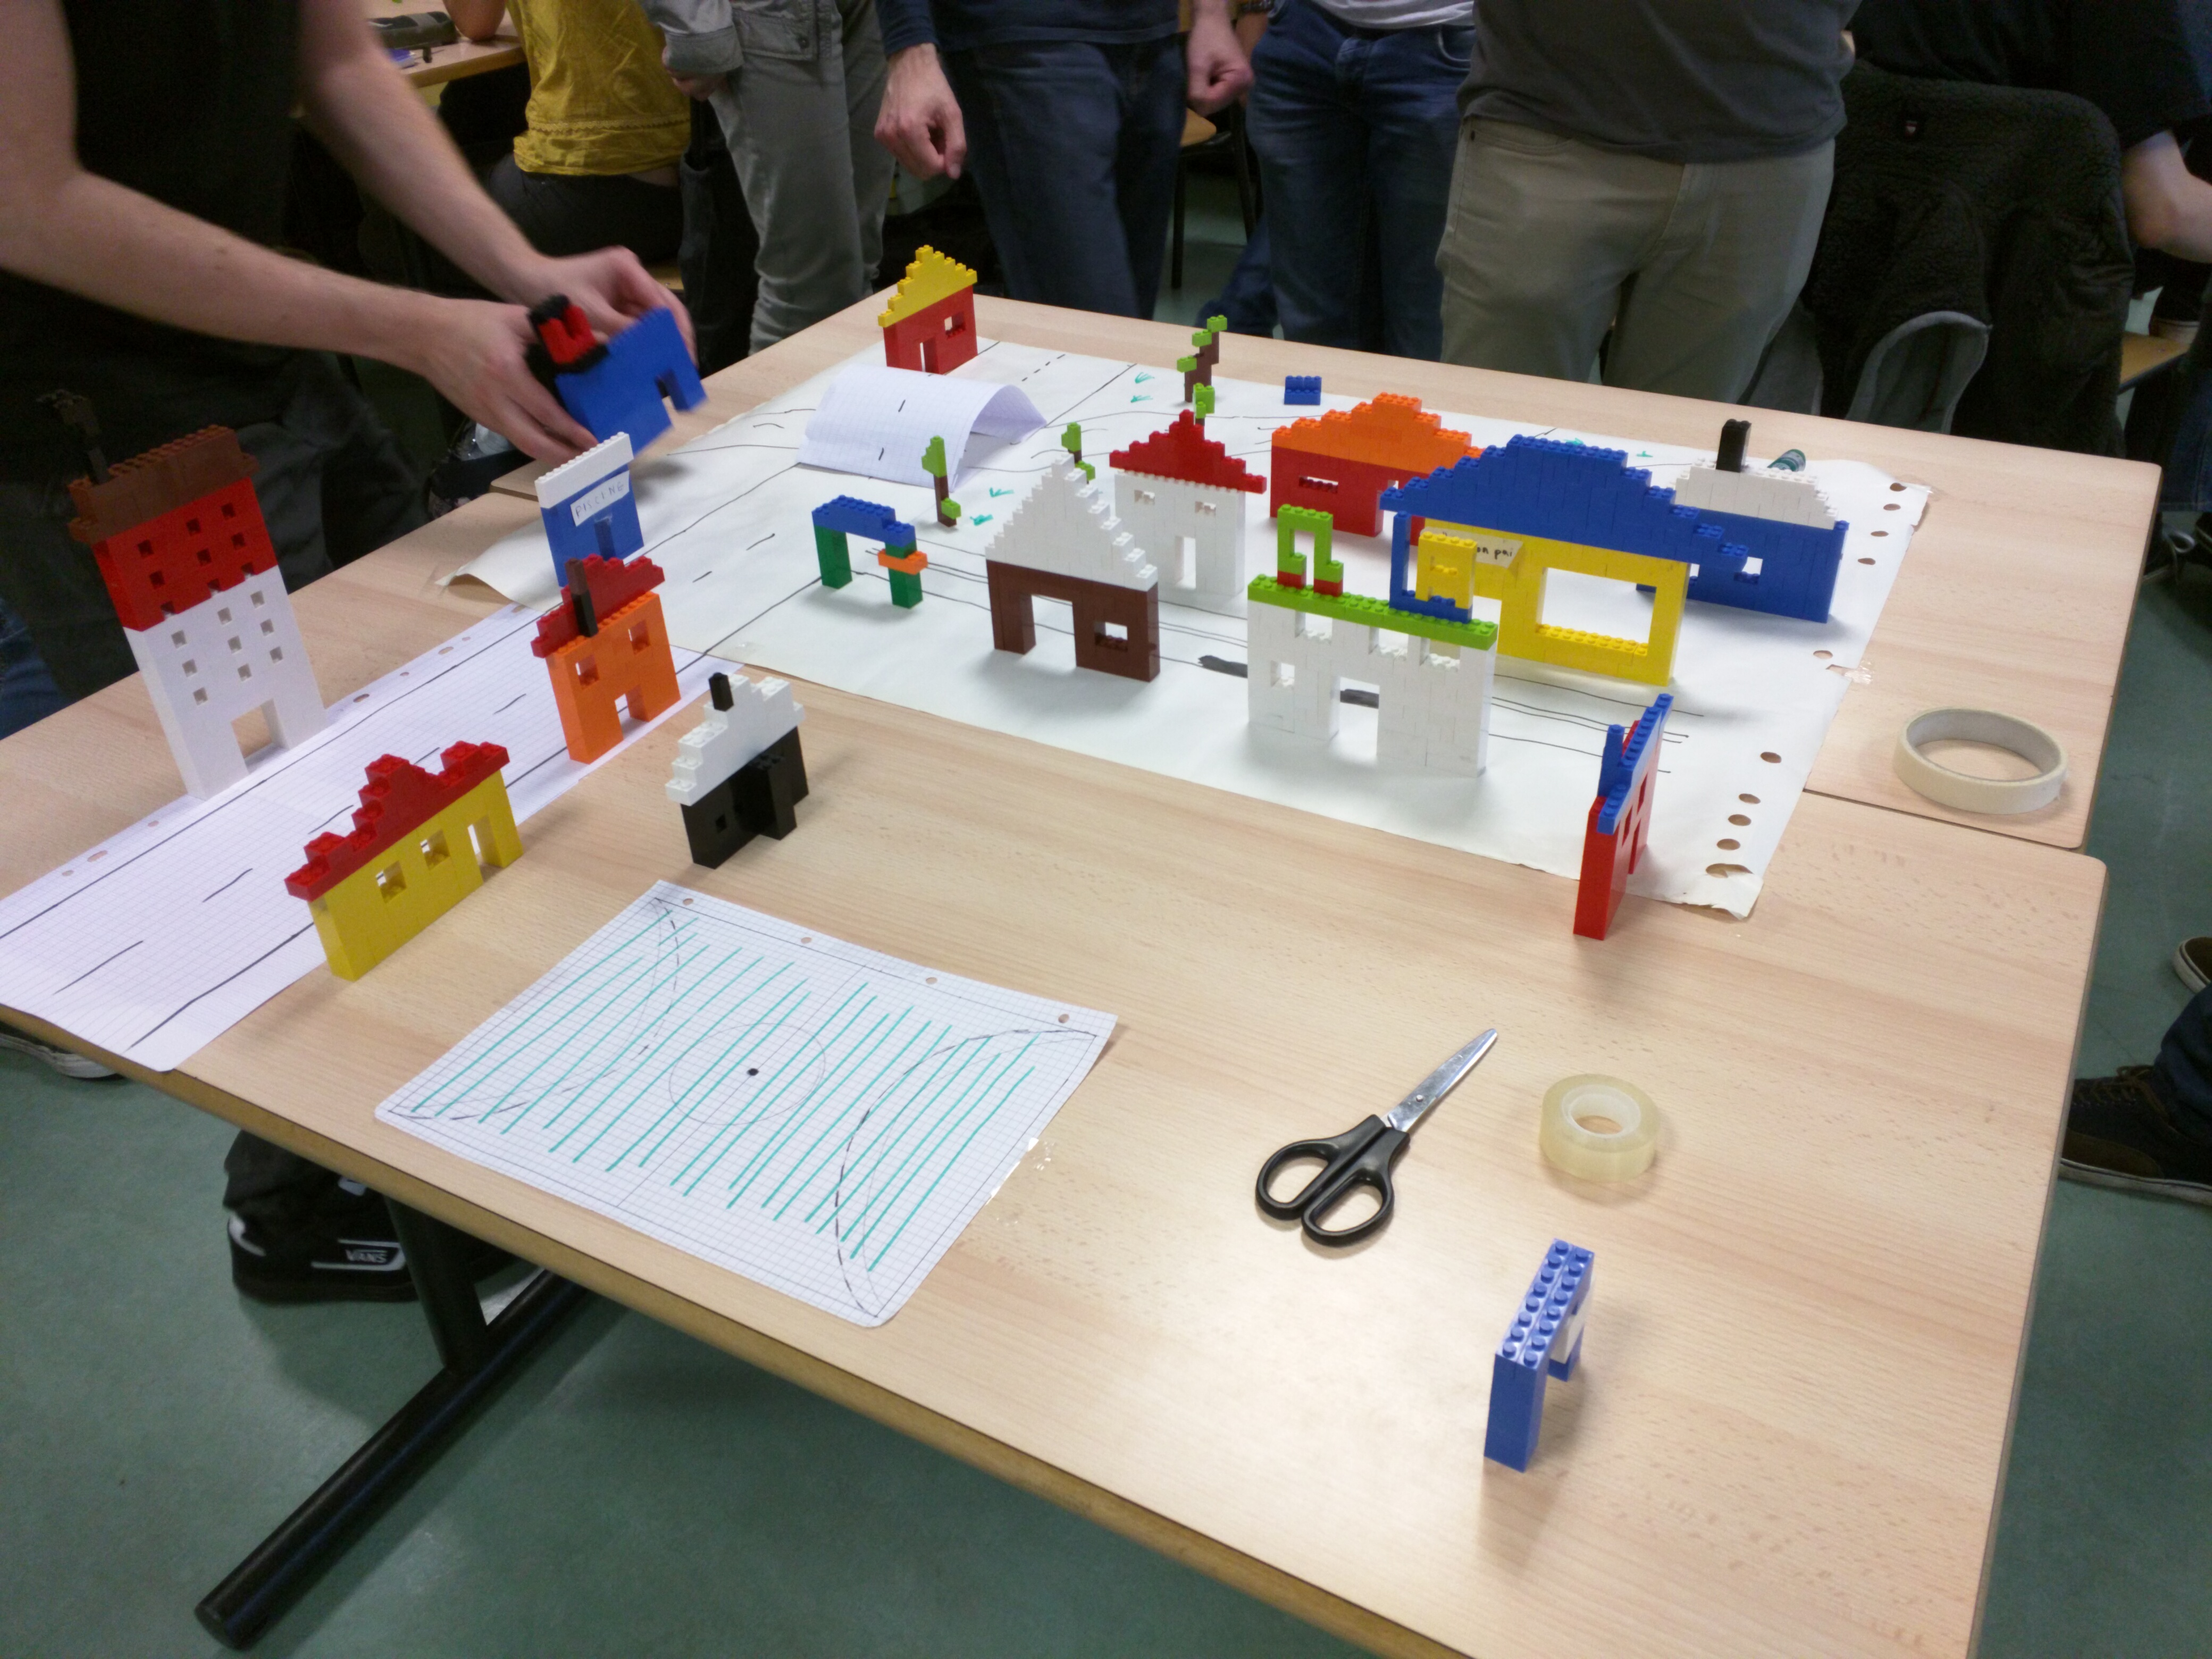
\includegraphics[width=\textwidth]{includes/201509_lego.jpg}      
      \end{center}
    \end{column}
    \begin{column}{0.5\textwidth}
  Objectifs : 
  \begin{itemize}
    \item créer de la cohésion dans la promotion
    \item plonger les étudiants dans le code après les vacances
  \end{itemize}
    \end{column}
  \end{columns}
\end{frame}

\begin{frame}{Septembre 2015 : Planning}
  \begin{center}
    \begin{tabular}{| c | c | c |}
      \hline
      \textbf{Jour 1} & \textbf{Jour 2} & \textbf{Jour 3}  \\
      \hline \hline
                      & sprint          & sprint           \\
      \hline
                      & sprint          & sprint           \\
      \hline \hline
      Lego4Scrum      & sprint          & soutenance       \\
      \hline
      sprint 0        & sprint          & rétro            \\
      \hline
    \end{tabular}
  \end{center}
    4 encadrants : les collègues poursuivent leur implication
\end{frame}

\subsection{Apprentissages}
\begin{frame}{Septembre 2015 : Apprentissages}
  \begin{columns}
    \begin{column}{0.5\textwidth}
      \begin{center}
        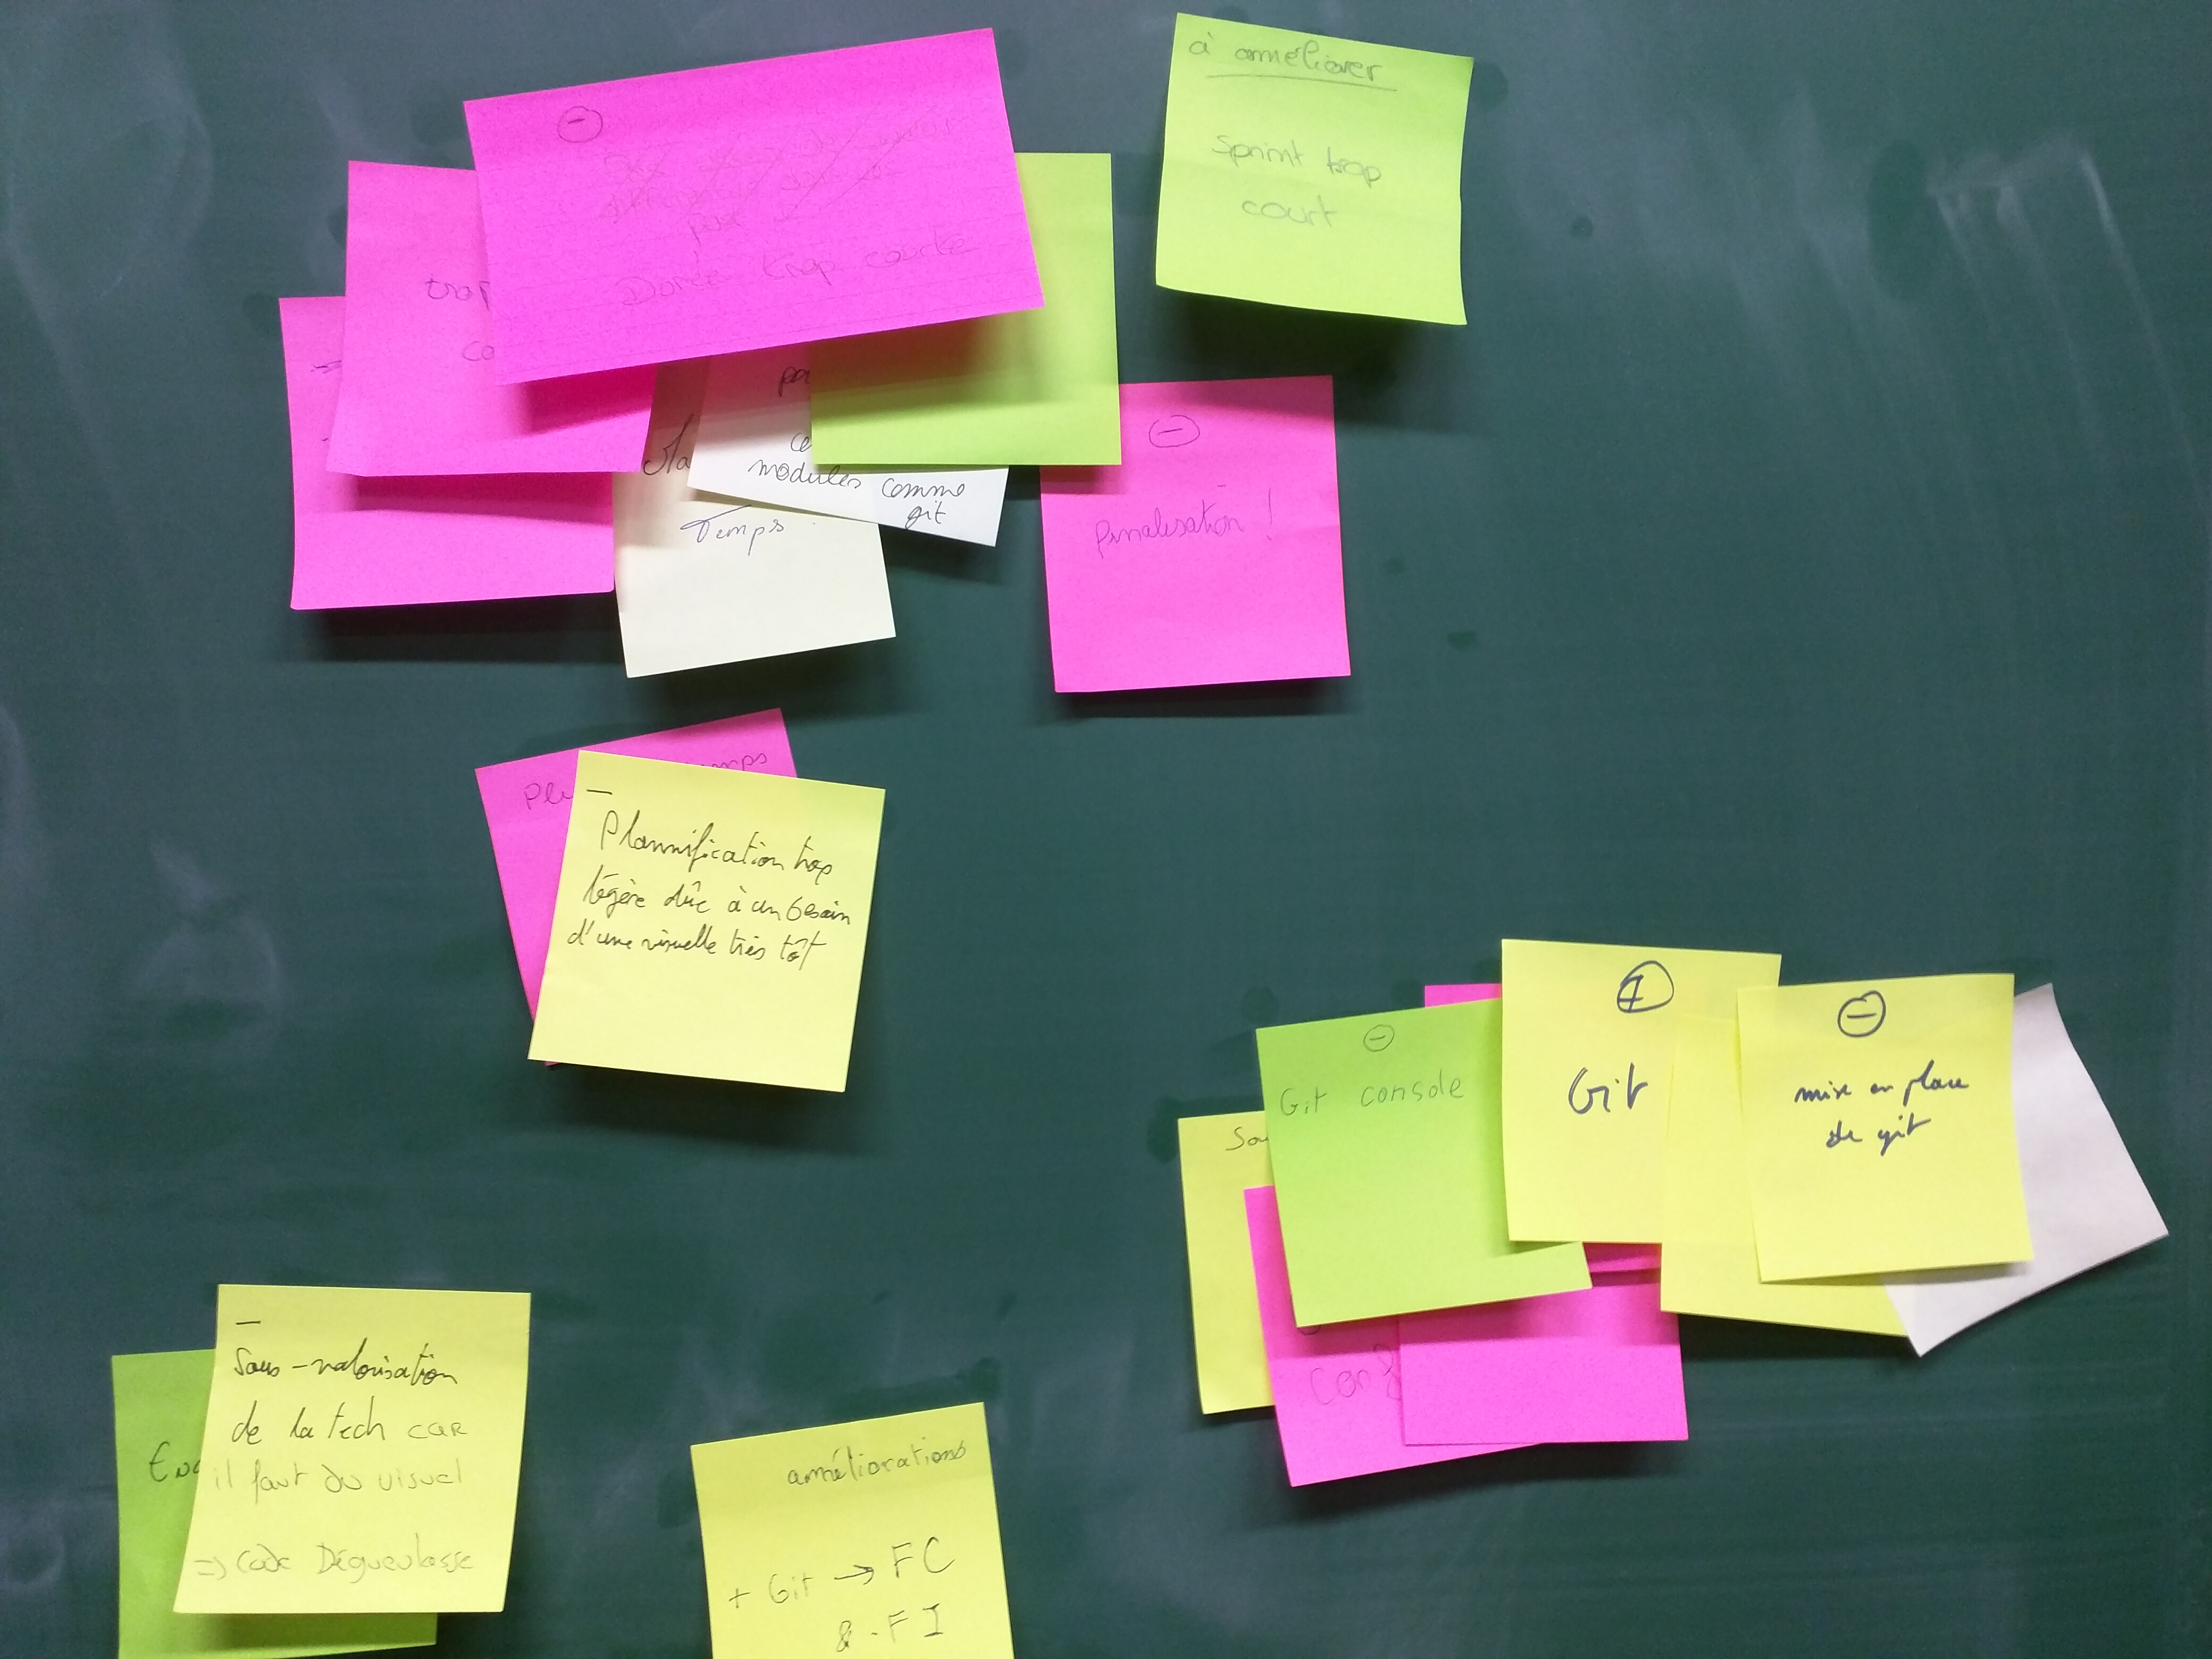
\includegraphics[width=\textwidth]{includes/201509_retro.jpg}      
      \end{center}
    \end{column}
    \begin{column}{0.5\textwidth}
  \begin{itemize}
    \item 2 jours et demis c'est très court
    \item les étudiants sont enthousiastes
    \item les enseignants aussi
  \end{itemize}
    \end{column}
  \end{columns}
\end{frame}

\section{Octobre 2015}
\subsection{Objectifs}
\subsection{Déroulement}
\begin{frame}{Octobre 2015 : Objectifs}
  \begin{columns}
    \begin{column}{0.5\textwidth}
      \begin{center}
        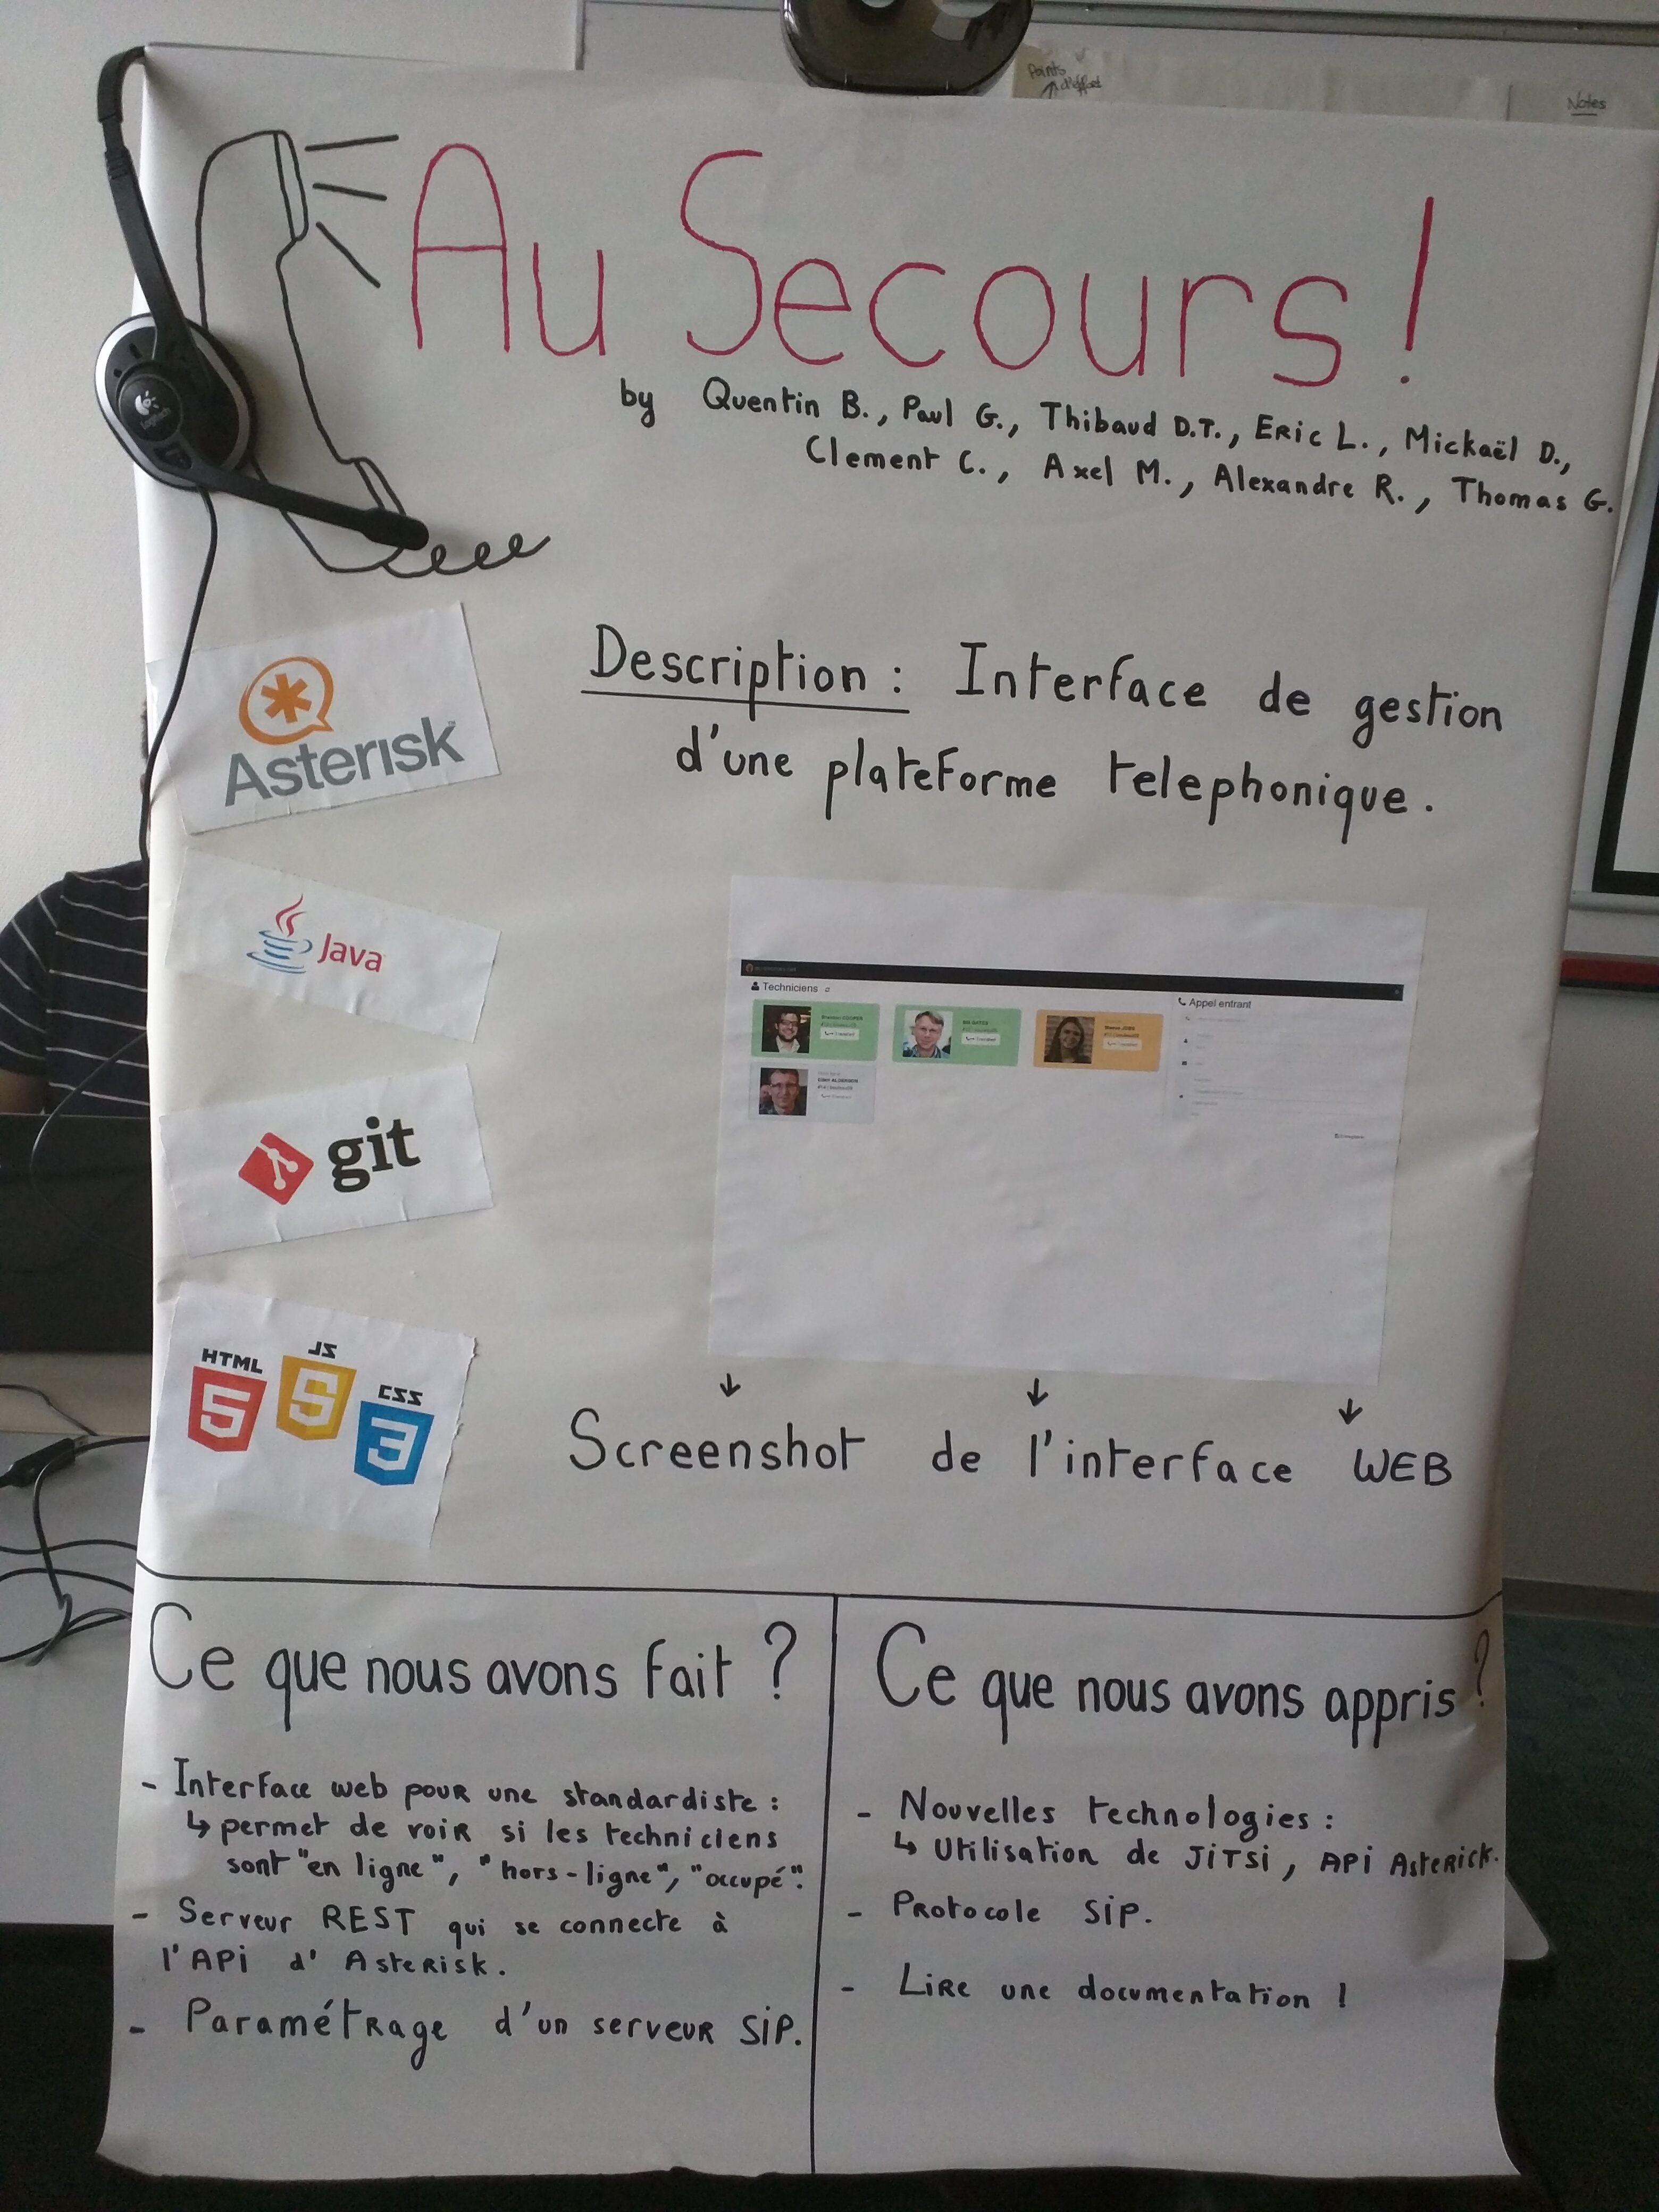
\includegraphics[width=\textwidth]{includes/201510_salon.jpg}      
      \end{center}
    \end{column}
    \begin{column}{0.5\textwidth}
      \begin{itemize}
        \item Objectif : valider la collaboration avec un porteur de projet
        \item Pas d'autres changement.
      \end{itemize}
    \end{column}
  \end{columns}
\end{frame}

\subsection{Apprentissages}
\begin{frame}{Octobre 2014 : Apprentissages}
  \begin{columns}
    \begin{column}{0.5\textwidth}
      \begin{center}
        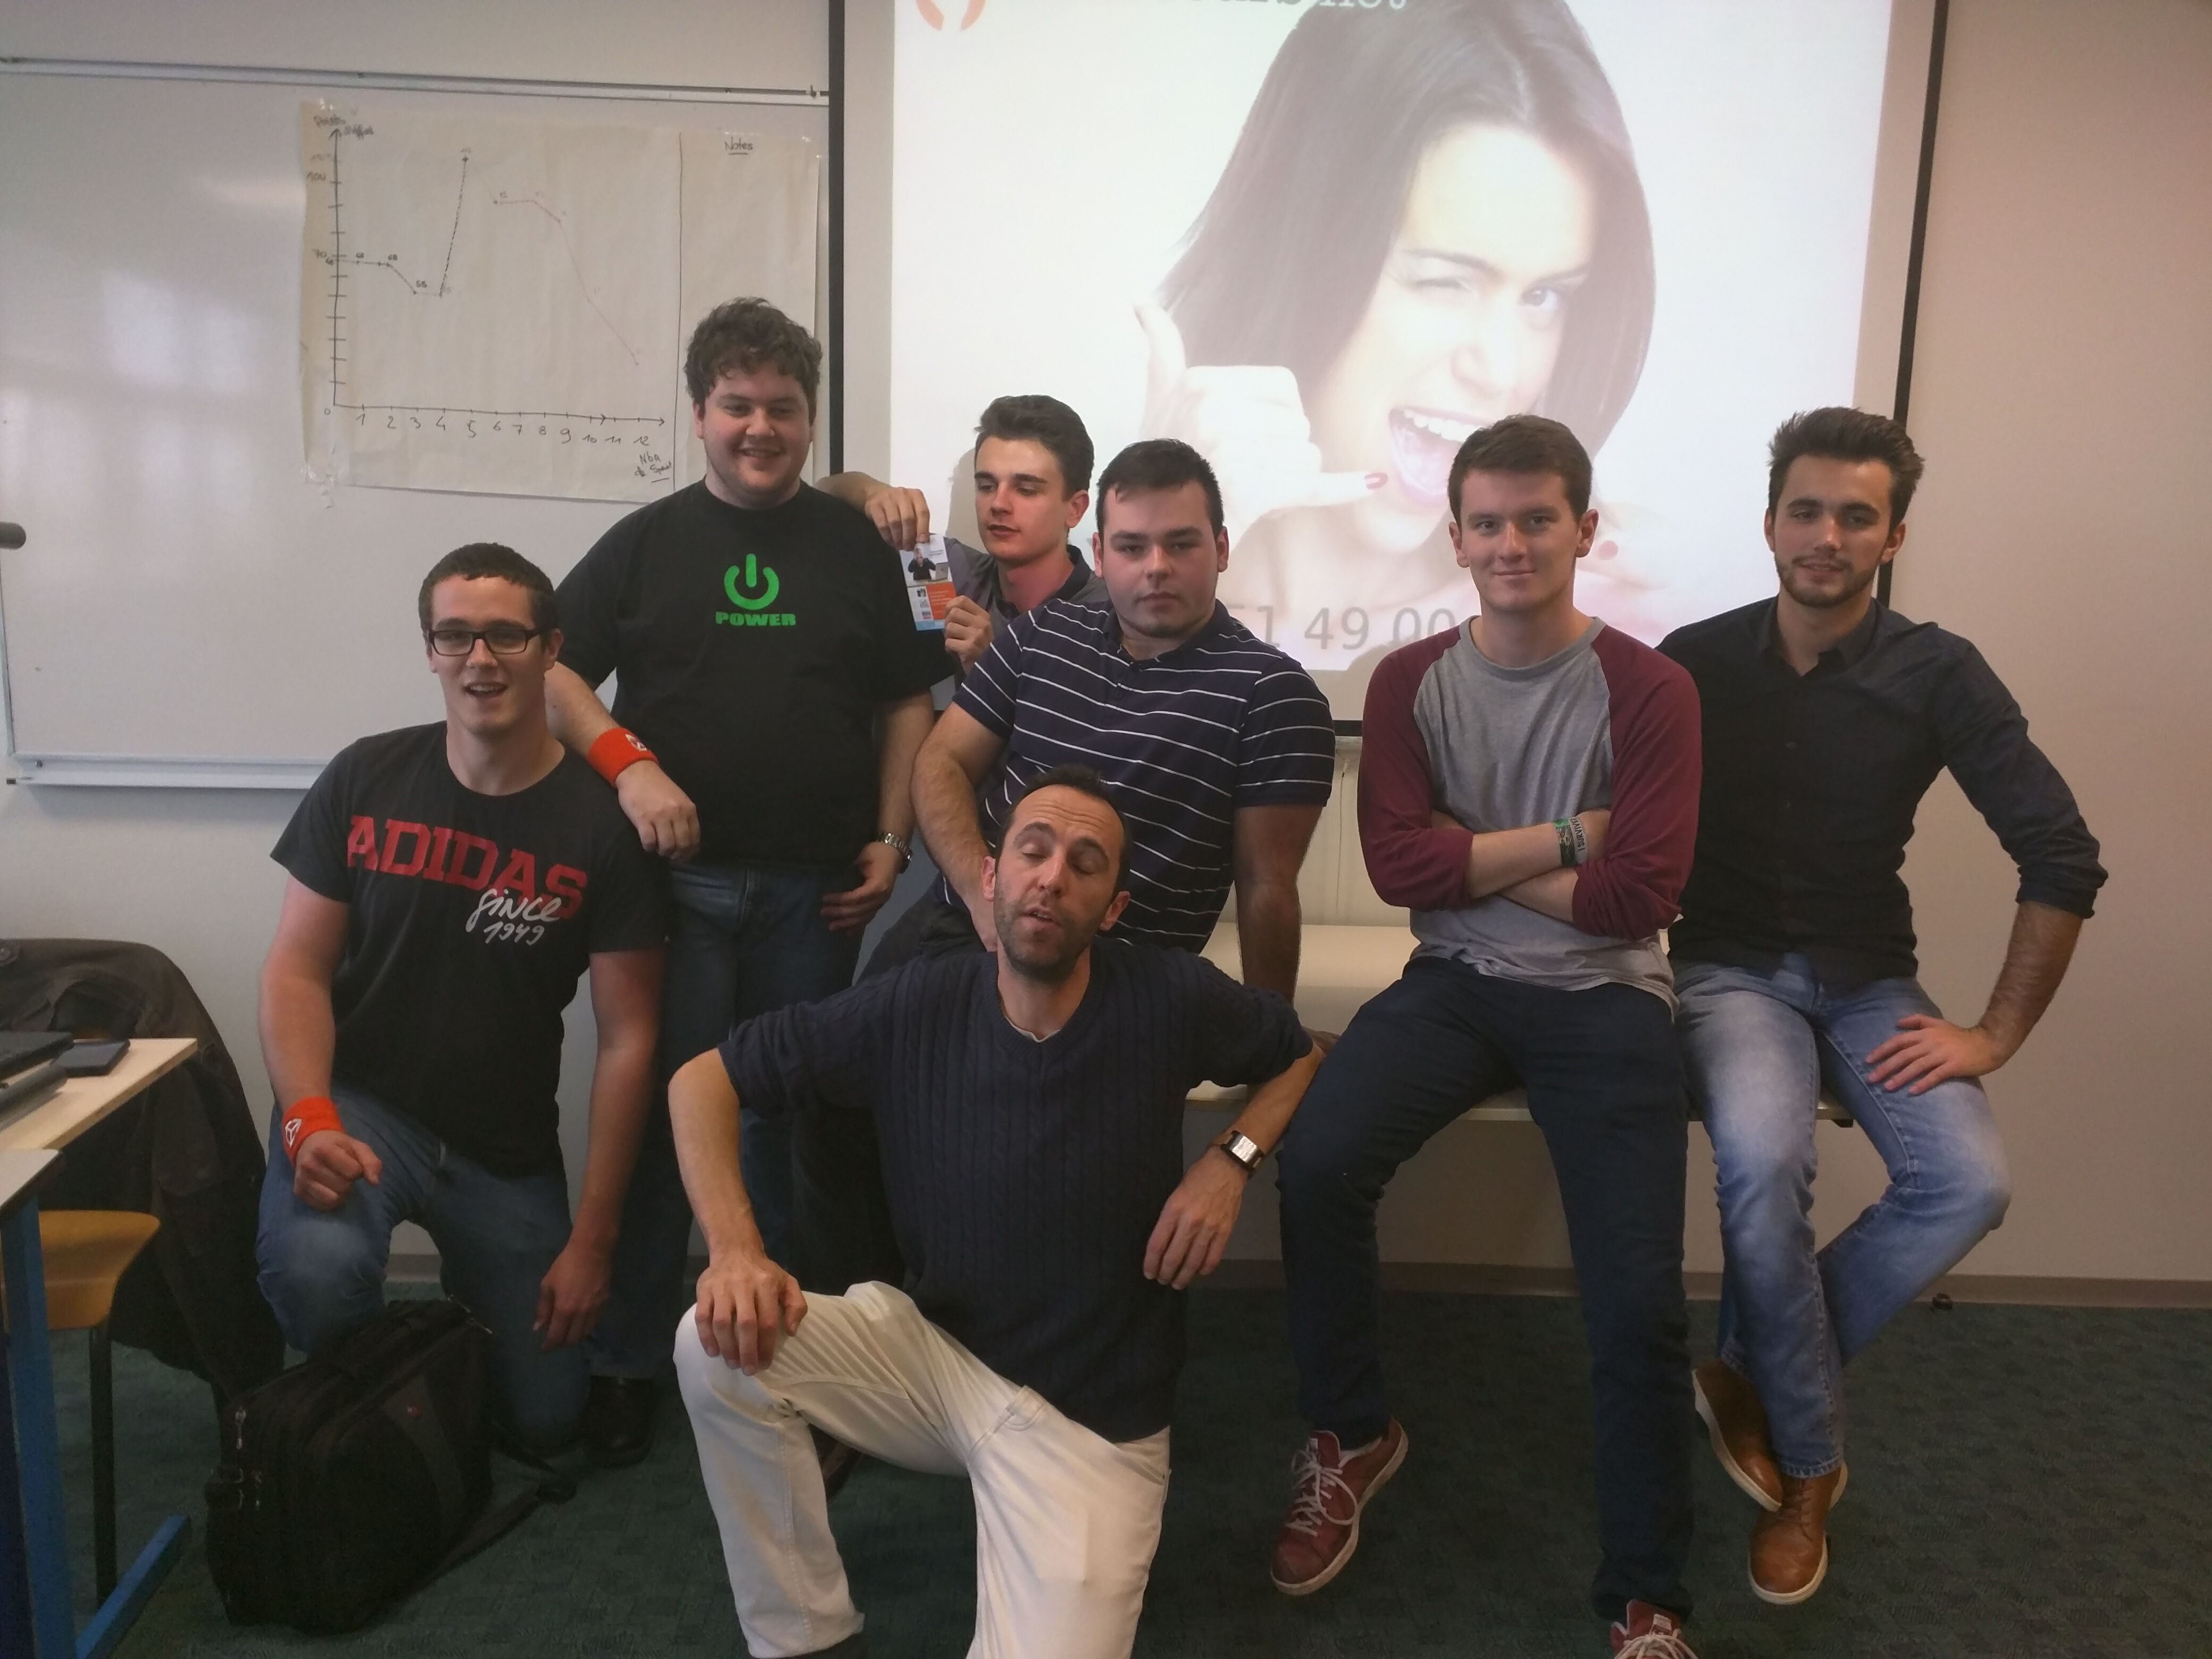
\includegraphics[width=\textwidth]{includes/201510_ausecours.jpg}      
      \end{center}
    \end{column}
    \begin{column}{0.5\textwidth}
      \begin{itemize}
        \item L'intégration du porteur de projet dès les premières minutes est un vrai succès
        \item Le porteur de projet était particulier
      \end{itemize}
    \end{column}
  \end{columns}
\end{frame}

\section{Mars 2016}
\subsection{Objectifs}
\begin{frame}{Mars 2016 : Expérience}
  Toute la promo en fin de S4 avec le groupe Euro des GEA.

  Objectifs : 
  \begin{itemize}
    \item valider la collaboration avec des entrepreneurs
    \item impliquer un autre département
  \end{itemize}
\end{frame}

\subsection{Déroulement}
\begin{frame}{Mars 2016 : Déroulement}
  \begin{itemize}
    \item 3 encadrants Info pour 3 groupes de TP Info (76 étudiants).
    \item 1 encadrant GEA pour 1 groupe de TP GEA
    \item 4 salles de TP
    \item constitution des équipes par les enseignants
    \item une demis journée pour présenter les projets puis 1 semaine de projet
  \end{itemize}
\end{frame}

\begin{frame}{Mars 2016 : Planning}
  \begin{center}
    \begin{tabular}{| c | c | c || c | c |}
      \hline
      \textbf{Jour 1} & \textbf{Jour 2} & \textbf{Jour 3} & \textbf{Jour 4} & \textbf{Jour 5} \\
      \hline \hline
      backlog         & sprint          & sprint          & sprint          & sprint          \\
      \hline
      sprint0 / lego  & sprint          & sprint          & sprint          & sprint          \\
      \hline \hline
      sprint          & sprint          & sprint          & sprint          & salon           \\
      \hline
      sprint          & sprint          & pitch           & sprint          & rétrospective   \\
      \hline
    \end{tabular}
  \end{center}
\end{frame}

\subsection{Apprentissages}
\begin{frame}{Mars 2016 : Apprentissages}
  \begin{itemize}
    \item avec 3 agilistes pour encadrer c'est plus facile
    \item la généralisation est un succès
    \item les étudiants sont enthousiastes
    \item l'activité est au bon moment ... sauf pour les concours
    \item le WE au milieu c'est reposant.
    \item 6 porteurs de projets c'est pas suffisant
  \end{itemize}
\end{frame}

\begin{frame}{Récapitulation}
  \begin{itemize}
    \item Janvier 2014 : 1 groupe de S3
    \item Octobre 2014 : 1 groupe de S4
    \item Janvier 2015 : toute la promo de S3
    \item Septembre 2015 : FI + FC
    \item Octobre 2015 : 1 groupe de S4
    \item Mars 2016 : info + GEA + porteur de projets
  \end{itemize}
\end{frame}

\section{Conclusion}
\begin{frame}{Et maintenant ?}
  \begin{itemize}
    \item Laurel et Hardy, l'aventure continue ?
    \item Étape cruciale du TDD en S3 ...
    \item Renforcement des liens GEA/INFO
      \begin{itemize}
        \item Intégrer les GEA en début de S3 (FI/FC),
        \item équipes communes lors de la journée de l'entreprenariat,
        \item final en beauté avec le projet agile de S4 !
      \end{itemize}
    \item ... et peut-être un jour: DU Lean startup ? :)
  \end{itemize}
\end{frame}

\end{document}

